\documentclass[a4paper, 18pt]{article} % A4 paper, readable font size
\usepackage{geometry} % Adjust margins
\geometry{top=0.8in, bottom=0.8in, left=0.8in, right=0.6in} 


% packages we'll need...

% for controlling page numbers
%\usepackage{fancyhdr}
%\pagestyle{fancy}
%\fancyhf{}
%\fancyhead[R]{\thepage}

% throw in page-top header
%\fancyhead[L]{The \textbf{Theory of Sequence Transformers} \& their \textbf{Statistics}}

% for graphics
\usepackage{graphicx}
\usepackage{caption}
\usepackage{float}

% for drawing text boxes

% for proper treatment of urls
\usepackage{hyperref}

% for tables
\usepackage{tabularx}

% for line-breaks in table cells
%\usepackage{makecell}

% for long tables
\usepackage{longtable}
% for custom table col widths
\usepackage{array}
\newcolumntype{L}{>{\centering\arraybackslash}m{2cm}}
\newcolumntype{M}{>{\centering\arraybackslash}m{5cm}}

% for json listings...
\usepackage{listings}
%\usepackage{minted}
%\usemintedstyle{xcode}% no parser errors in listings?
%\usemintedstyle{bw} % grayscale color in listings, but shows parser errors!

% for maths
\usepackage{amsmath}
% for number sets symbols
\usepackage{amssymb}
%\usepackage{ntheorem}
\usepackage{amsthm}

% extra symbols
\usepackage{textgreek}
%\usepackage{mnsymbol}

% for writing our theorems and defs...
\newtheorem{comp}{Computation}
\newtheorem{theo}{Theorem}
\newtheorem{defn}{Definition}
\newtheorem{lem}{Lemma}
\newtheorem{prop}{Proposition}
\newtheorem{axiom}{Axiom}
\newtheorem{post}{Postulate}
\newtheorem{trans}{Transformation}
\newtheorem{transf}{Transformer}

% for highlighting text
\usepackage{xcolor, soul}
\definecolor{highcolor}{rgb}{0,255,255} %a color for background, that is friendly on black text foreground
\sethlcolor{highcolor}


% for wrapping text around floats
\usepackage{wrapfig}

% to include pdf pages
\usepackage{pdfpages}

% for multiline comments...
\newcommand{\comment}[1]{}

% for the cardinality symbol
\newcommand{\invpi}{\rotatebox[origin=c]{180}{$\pi$}}

\title{TEA RESEARCH: \textbf{TEA ON THE WEB} \\[0.5ex] \small A High-Level Web Software Operating Environment Specification 
For The TEA Programming Language:\\ Web TEA Architecture
}


\author{Joseph Willrich Lutalo\thanks{Also inventor of the TEA text-processing oriented General-purpose Computer Programming Language ---\\ \url{https://github.com/mcnemesis/cli_tttt}}\\
\texttt{joewillrich@gmail.com, jwl@nuchwezi.com}}


\begin{document}

\maketitle


\Large

\begin{abstract}
\large

Expressed as the combination of 3 environments --- the local-browser/system environment, the TEA runtime environment, and the web/external environment --- into a single, overall Software Operating Environment\cite{lutalo2020dnap} for the TEA programming language, this is \textbf{the planned architecture for executing TEA programs within a web browser context on any device or technology platform or basically over the web}. It is intended as the next generation and \textbf{alternative reference implementation} for the \textbf{Transforming Executable Alphabet}(TEA) language that is to be built with [vanilla] JavaScript as the base/host language instead of Python 3 that currently powers the command-line reference implementation of TEA\cite{lutalo2024software}\cite{teaproject} installable on Linux, Debian-package compliant Operating Systems as well as anywhere Python 3 source-code can run. This implementation shall attempt to support the complete TEA Instruction Set as currently specified in the TAZ\cite{Lutalo2024TEATAZ}. Ultimately, this implementation shall make it simple and readily possible for the TEA language to be used by netizens or anyone able to access the Internet or use a standard web-browser such as Firefox, Google Chrome or Safari. Such a break-through would then also allow us to see such important and generally useful programs such as ZHA\cite{jwlzha} being able to run in any web-browser or basically over the web, but also, researchers and especially mathematical scientists interested in practically exploring or applying the newly proposed field of transformatics\cite{lutalo2025sequence}, shall then be able to do so, from the comfort of their web-browsers and not the command-line as is currently possible.
     \newline\newline
     \textbf{Keywords}: Software Language Engineering, Software Operating Environment, TEA, Web, JavaScript
\end{abstract}


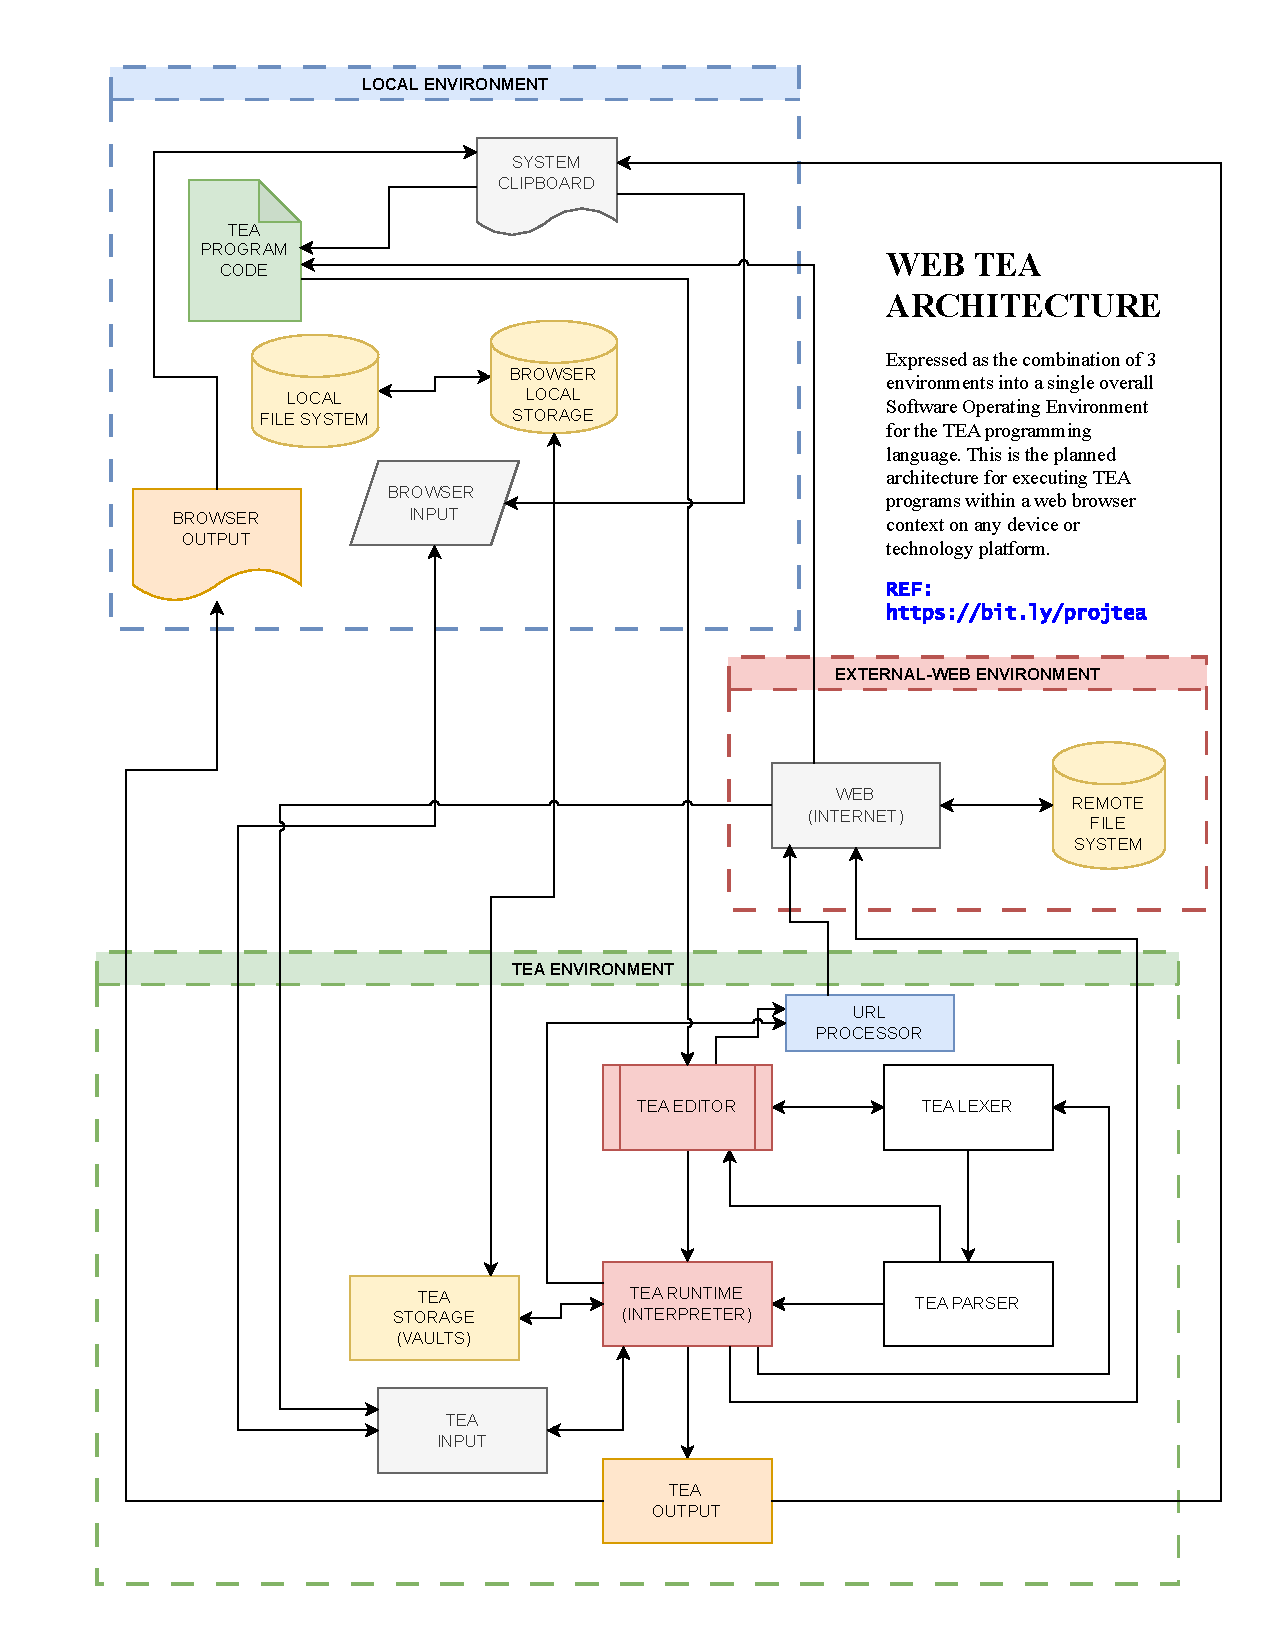
\includepdf[pages=1]{resources/webtea_arch.pdf}

\bibliographystyle{unsrt}
\bibliography{references}


\end{document}
